% !TEX root = thesis.tex

\chapter{Additional graphs}
\label{app:graphs}
%This section shows additional graphs. 
%\section{Fits to $\jt{}$ signal}
\begin{figure}[h!]
\centering
%\begin{subfigure}{0.24\textwidth}
%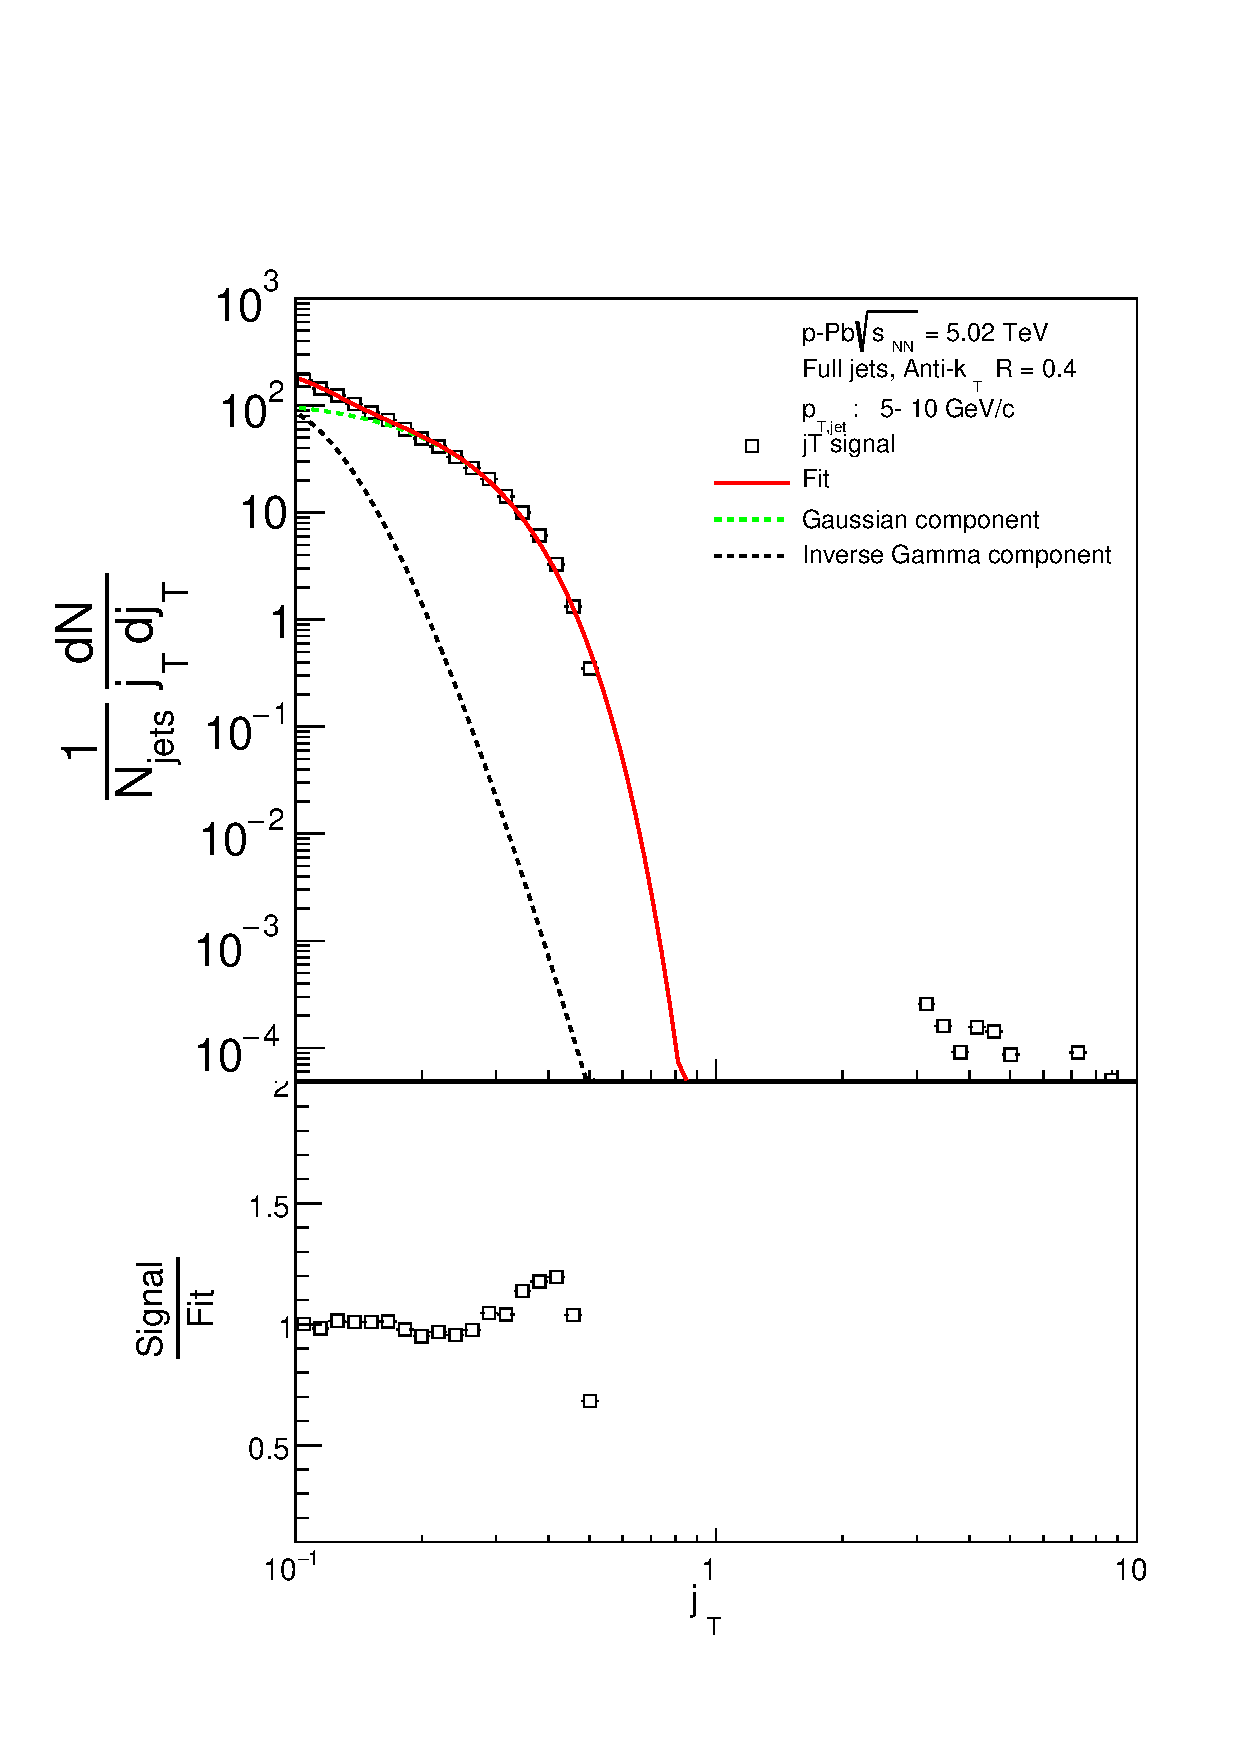
\includegraphics[width=0.95\textwidth]{results/JetConejTSignalFit/JetConejTSignalFitNFin00JetPt00perconeBgBayes}
%\end{subfigure}
%\begin{subfigure}{0.24\textwidth}
%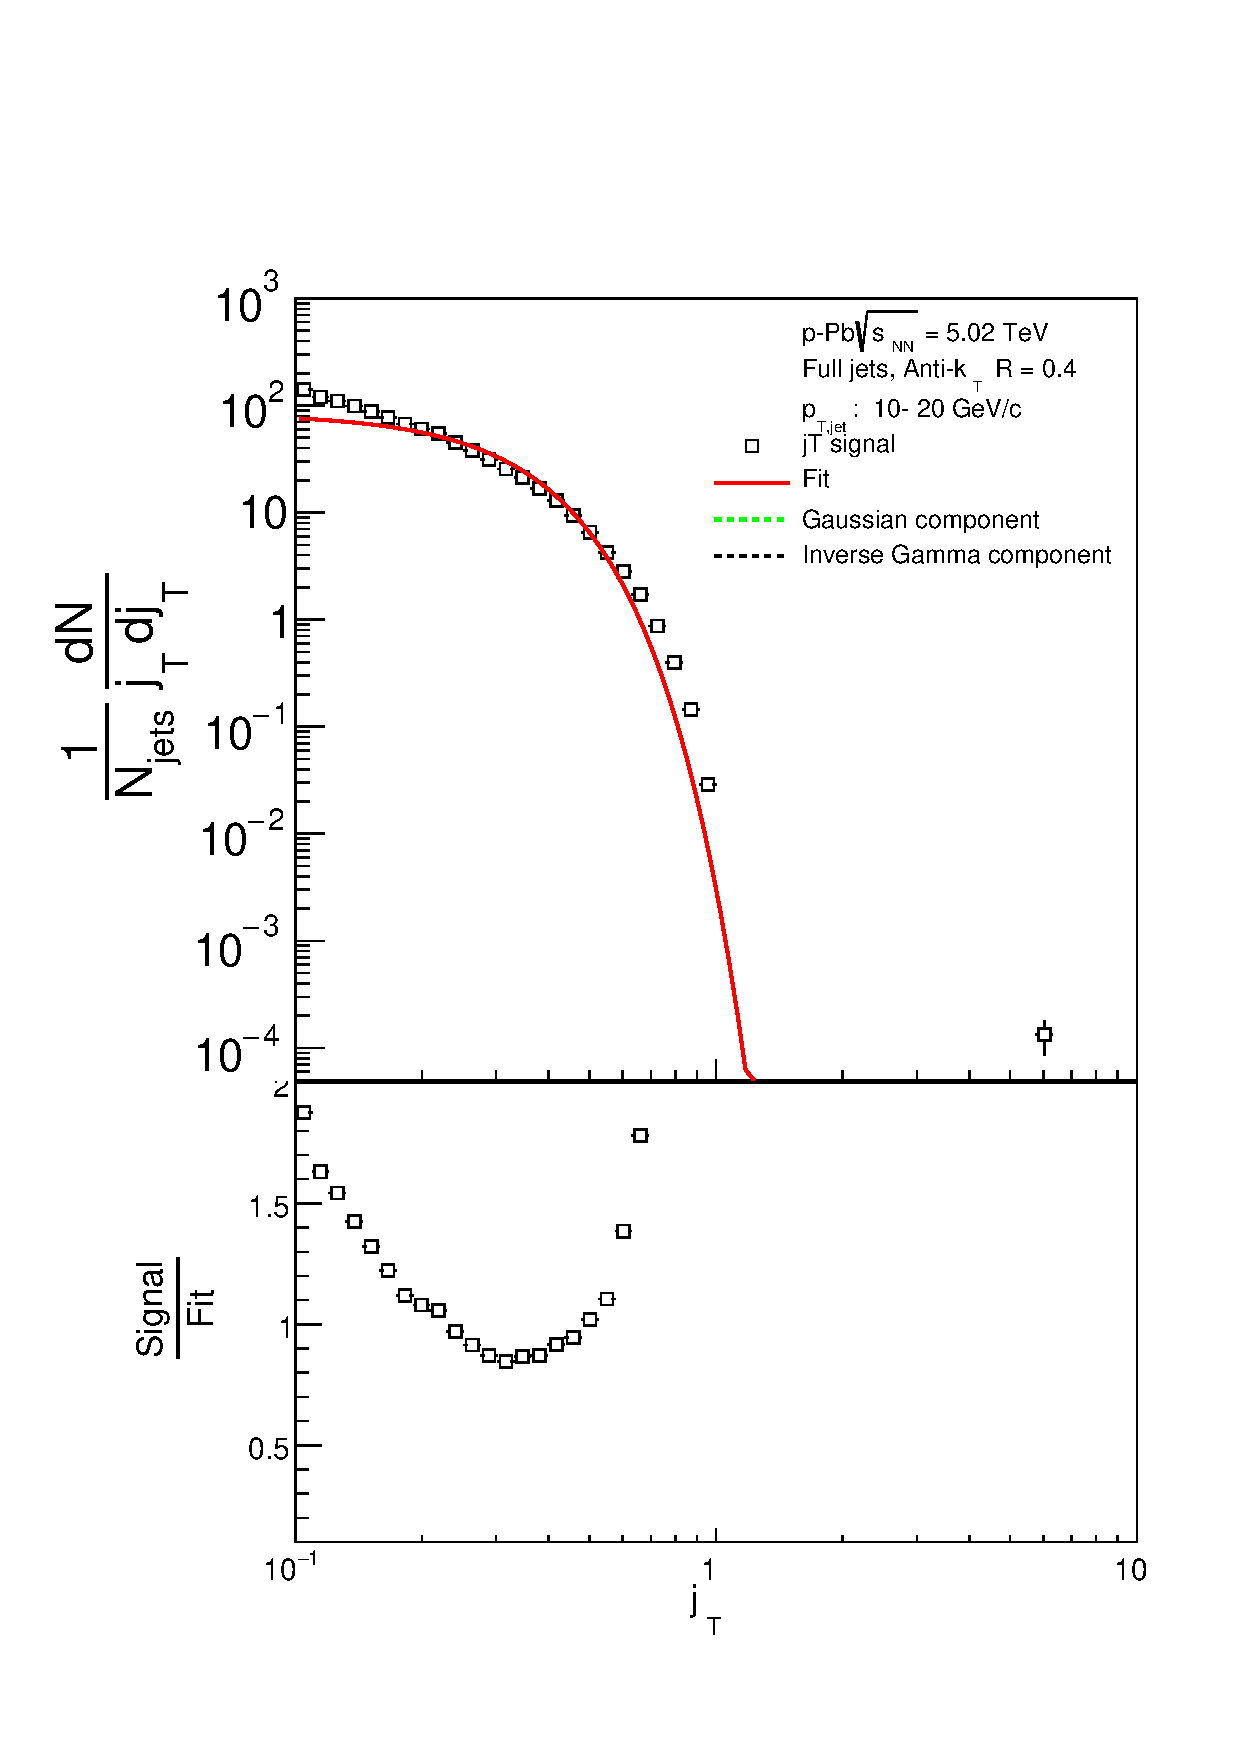
\includegraphics[width=0.95\textwidth]{results/JetConejTSignalFit/JetConejTSignalFitNFin00JetPt01perconeBgBayes}
%\end{subfigure}
%\begin{subfigure}{0.24\textwidth}
%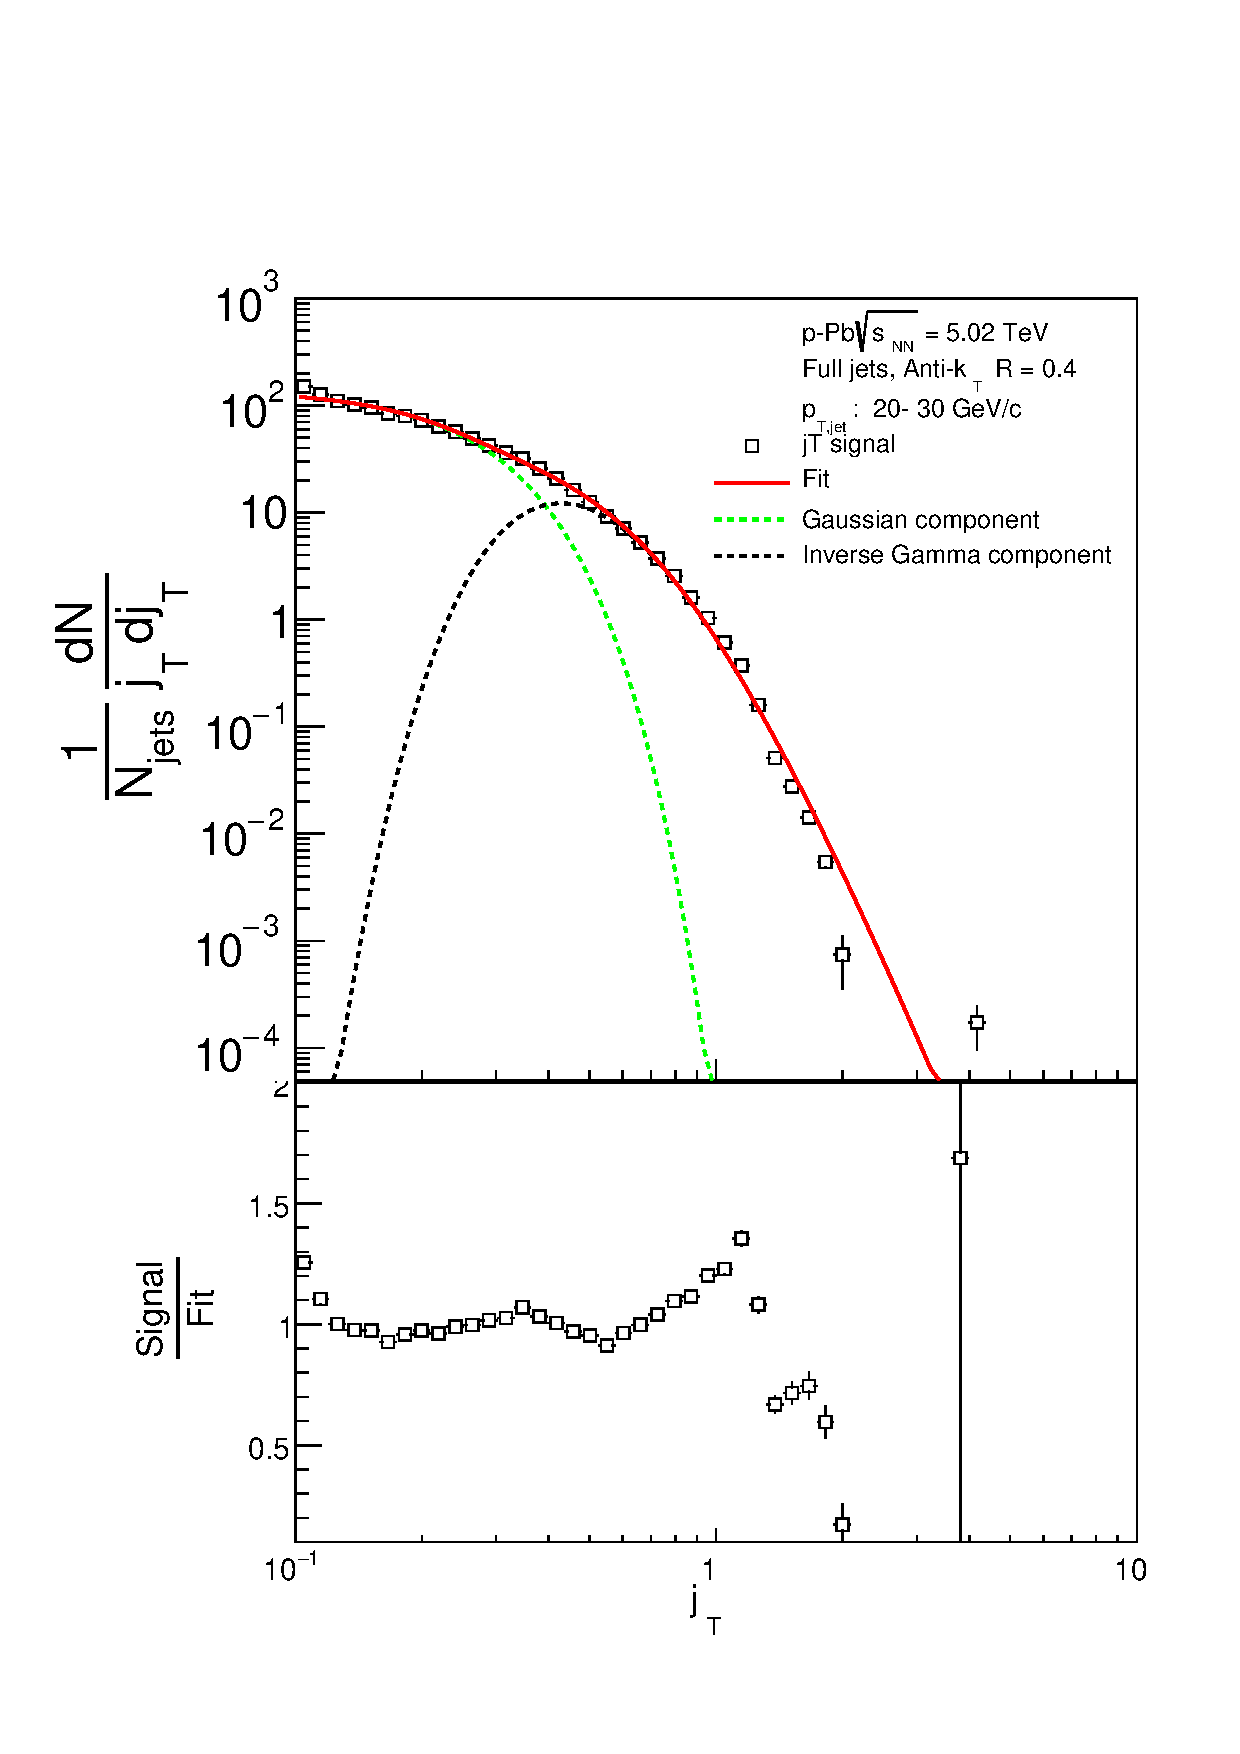
\includegraphics[width=0.95\textwidth]{results/JetConejTSignalFit/JetConejTSignalFitNFin00JetPt02perconeBgBayes}
%\end{subfigure}
\begin{subfigure}{0.36\textwidth}
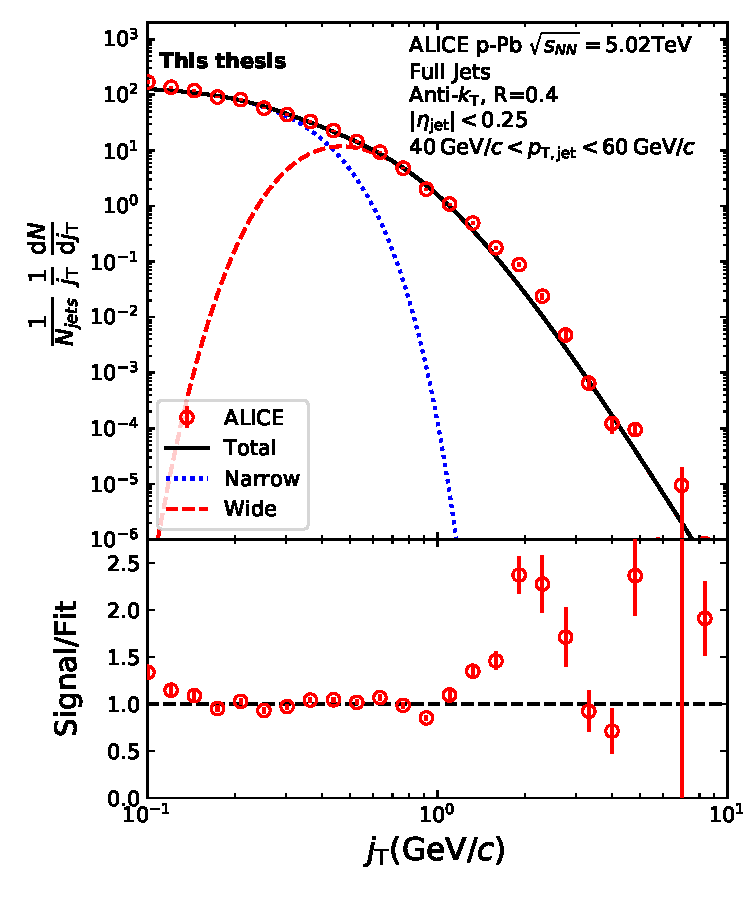
\includegraphics[width=0.99\textwidth]{figures/results/JtSignalFinalFitJetPt4}
\end{subfigure}
\begin{subfigure}{0.36\textwidth}
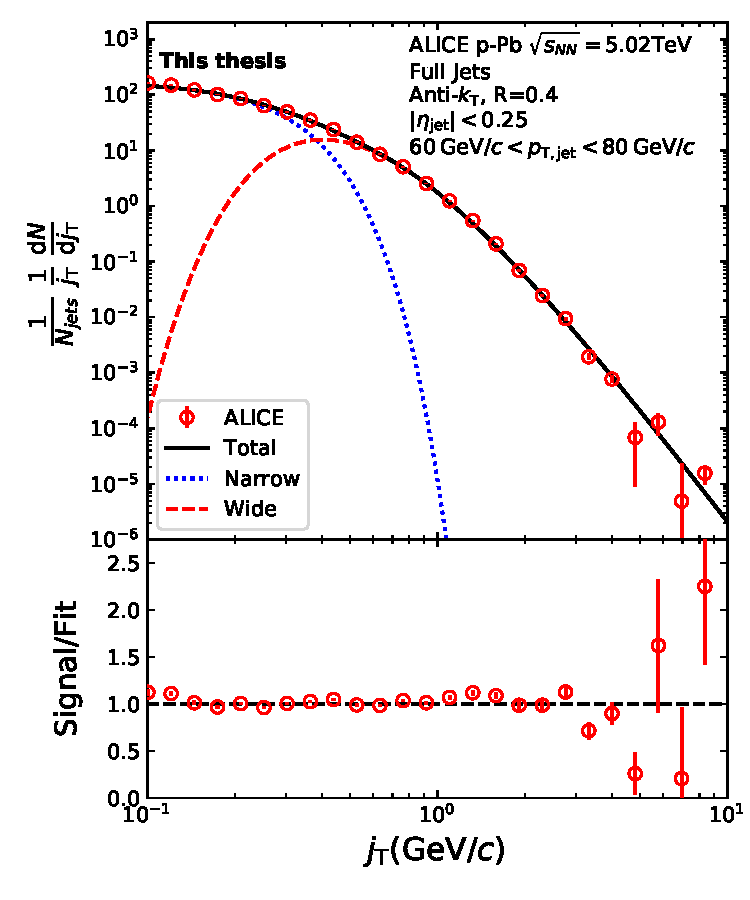
\includegraphics[width=0.99\textwidth]{figures/results/JtSignalFinalFitJetPt5}
\end{subfigure}
\begin{subfigure}{0.36\textwidth}
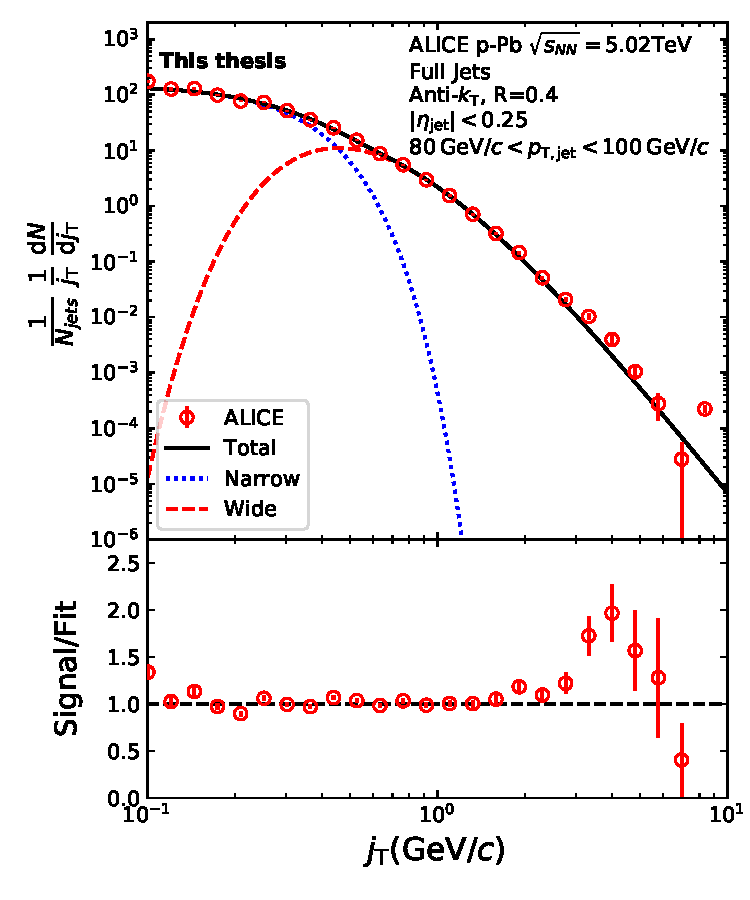
\includegraphics[width=0.99\textwidth]{figures/results/JtSignalFinalFitJetPt6}
\end{subfigure}
\begin{subfigure}{0.36\textwidth}
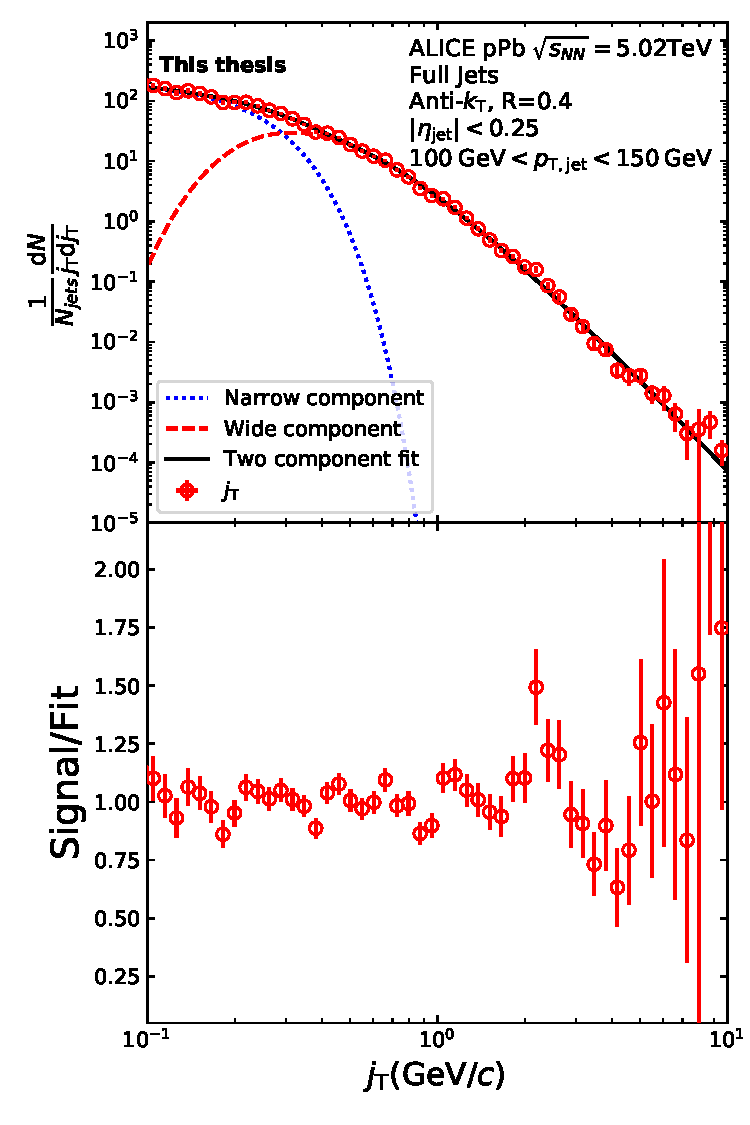
\includegraphics[width=0.99\textwidth]{figures/results/JtSignalFinalFitJetPt7}
\end{subfigure}
\caption{$\jt{}$ signal fits in different jet $\pt{}$ bins}
\label{fig:fits3}
\end{figure}

%\FloatBarrier
%\section{Monte Carlo comparisons}
%\label{app:mc}

\begin{figure}[h!]
\centering
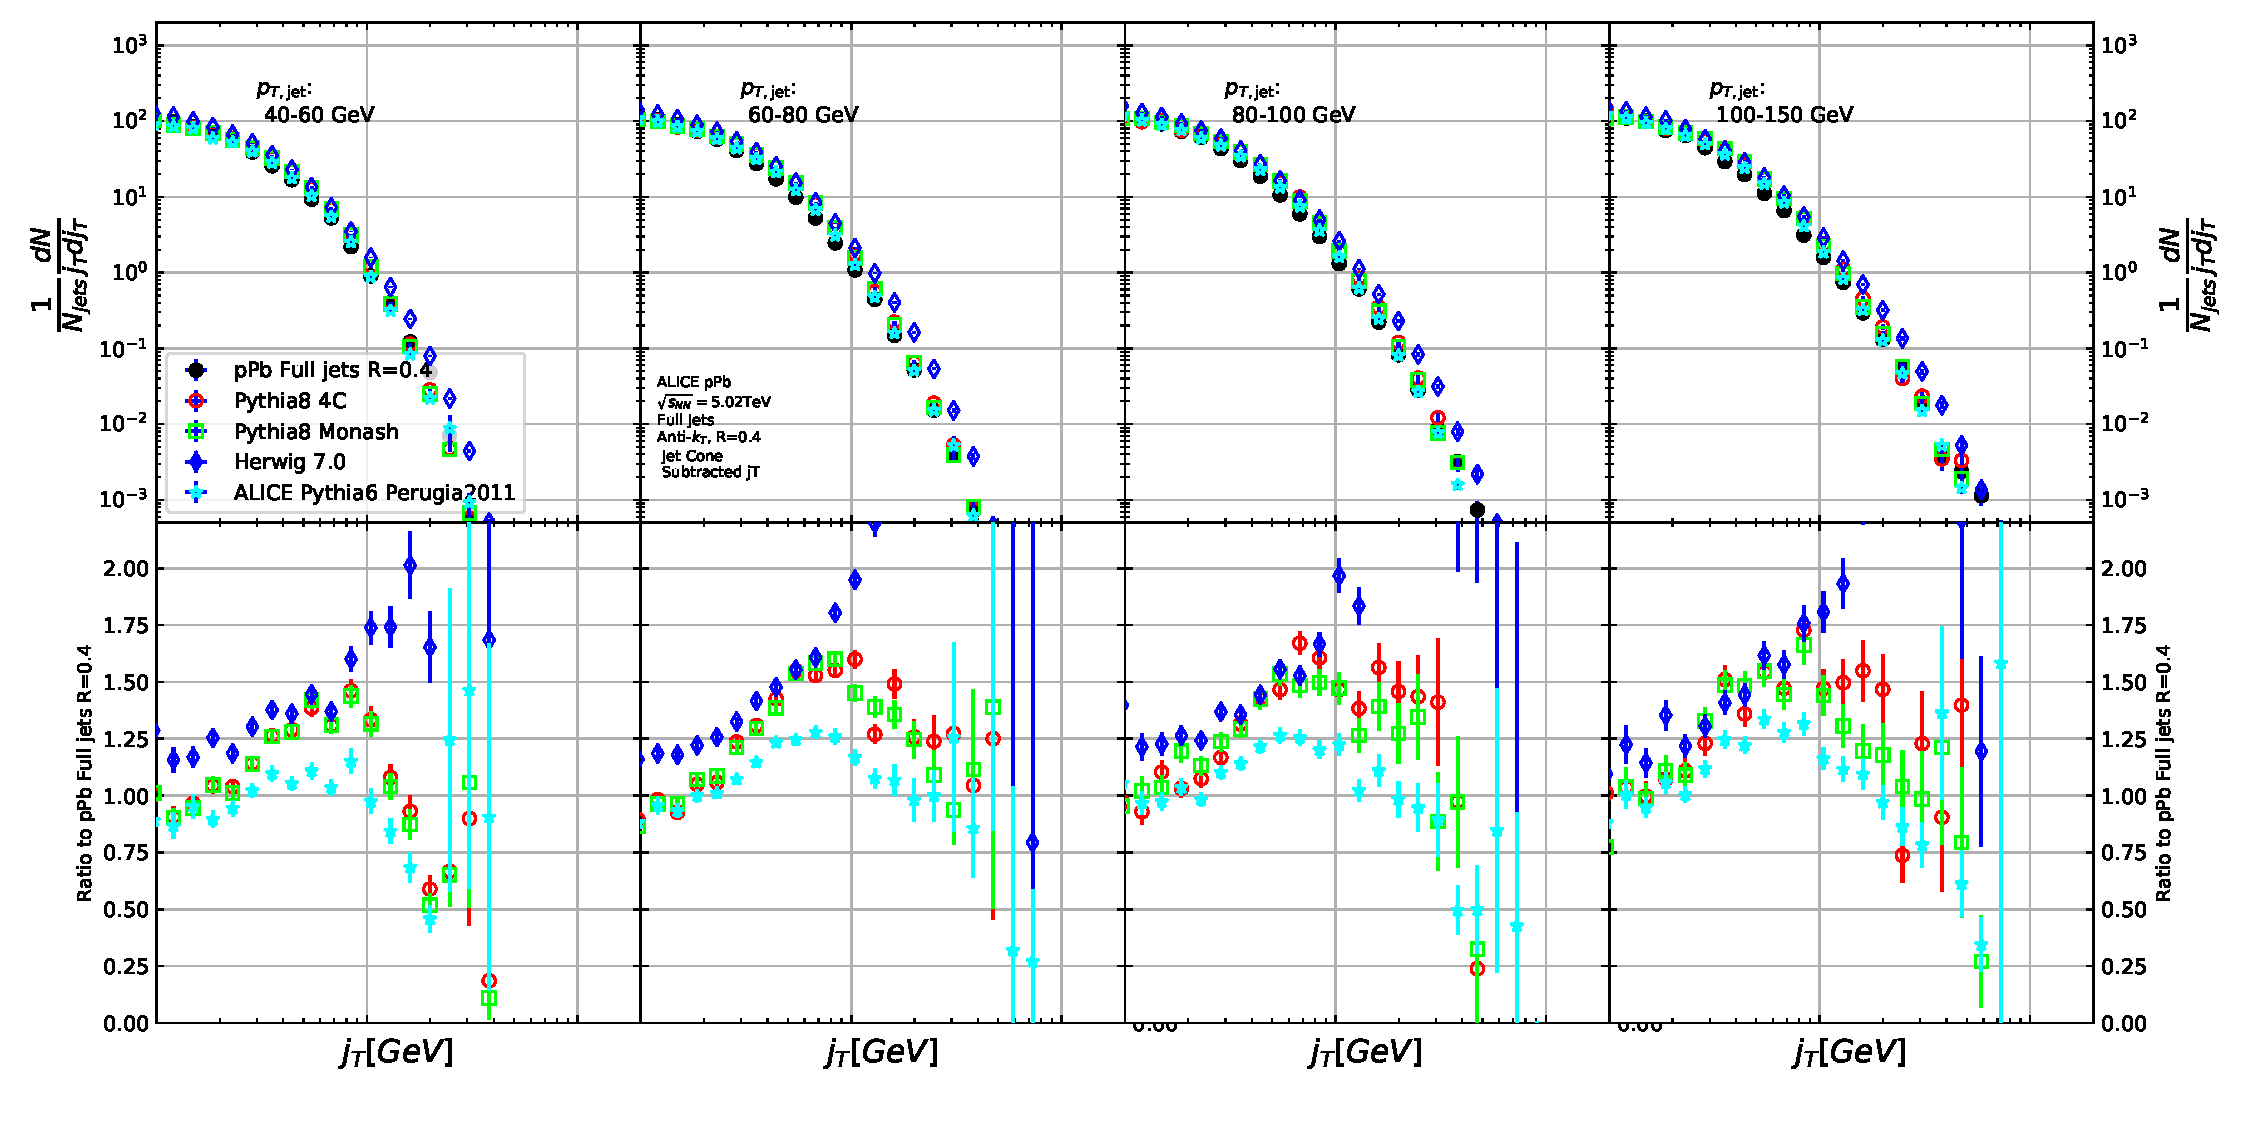
\includegraphics[width=0.95\textwidth]{figures/results/PythiaR04JetConeJtSignalPtFrom3To8.pdf}
\label{fig:mc3}
\caption{Figure shows comparisons of $\jt{}$ signals between ALICE data and various Monte Carlo simulations.
}
\end{figure}
